\documentclass[11pt]{article}

\usepackage[margin=1in]{geometry}
\usepackage{amsmath,amssymb,bm}
\usepackage{booktabs}
\usepackage{tabularx}
\usepackage{graphicx}
\usepackage{xcolor}
\usepackage{listings}
\usepackage[colorlinks=true,linkcolor=blue!50!black,citecolor=blue!50!black,
  urlcolor=blue!50!black]{hyperref}

\graphicspath{{../paper/figs/}}
\setlength{\parindent}{0pt}
\setlength{\parskip}{0.55em}
\setlength{\emergencystretch}{2em}

\definecolor{codebg}{RGB}{246,247,249}
\definecolor{codecomment}{RGB}{70,105,75}
\lstset{
  basicstyle=\ttfamily\small,
  backgroundcolor=\color{codebg},
  commentstyle=\color{codecomment},
  columns=fullflexible,
  frame=single,
  framerule=0.25pt,
  keepspaces=true,
  showstringspaces=false,
  breaklines=true,
  xleftmargin=0.4em,
  framexleftmargin=0.4em
}

\newcommand{\Jzz}{J_{zz}}
\newcommand{\Jpm}{J_{\pm}}
\newcommand{\bq}{\bm q}
\newcommand{\btheta}{\bm\theta}
\newcommand{\PP}{\mathcal P}
\newcommand{\cQ}{\mathcal Q}
\newcommand{\code}[1]{\texttt{#1}}

\title{A Pedagogical Guide to Transport-Projected Exact Diagonalization\\
for Quantum Spin Ice}
\author{Implementation note for the \code{twist\_qsi\_demo} repository}
\date{\today}

\begin{document}
\maketitle

\begin{abstract}
This note explains the transport-projected band protocol at the level needed
to reproduce, audit, and extend its current implementation.  The central
problem is that a small periodic pyrochlore cluster contains ice-preserving
virtual paths that close only through a periodic image.  On cubic-16, a
spurious four-spin process then appears at order $\Jpm^2/\Jzz$, parametrically
before the contractible six-spin ring exchange at order
$|\Jpm|^3/\Jzz^2$~\cite{Hermele2004}.  The protocol labels each completed virtual path by its
transport in the covering lattice and projects the selected low-energy band
onto zero transport.  The production campaign now uses exact microscopic
eigenspaces and a polar pullback on matched $M=2,3,4$ character grids; the
$M=3\to4$ centered operator change is 0.498\%.  The order-two/order-three row
enumeration remains only a pedagogical and topological diagnostic.
\end{abstract}

\tableofcontents

\section{What problem is being solved?}

The local-axis XXZ model is
\begin{equation}
 H=H_0+V=
 \Jzz\sum_{\langle ij\rangle}S_i^zS_j^z
 -\Jpm\sum_{\langle ij\rangle}
 \left(S_i^+S_j^-+S_i^-S_j^+\right).
 \label{eq:model}
\end{equation}
At $\Jpm=0$, the low-energy model space $P$ is the spin-ice manifold: every
tetrahedron has two spins up and two down.  In the thermodynamic lattice, the
first off-diagonal process within this manifold is the six-spin ring exchange
around a contractible pyrochlore hexagon, with scale
\begin{equation}
 g_6=12\frac{|\Jpm|^3}{\Jzz^2}.
\end{equation}

A periodic finite cluster has an additional possibility.  A sequence may
return to the same finite-cell spin configuration while transporting spin
through a nonzero supercell image.  Cubic-16 consequently admits
ice-preserving four-loops with scale
\begin{equation}
 g_4=4\frac{\Jpm^2}{\Jzz}.
\end{equation}
This is a finite-topology artifact, not a local bulk plaquette.  Because it is
lower order than $g_6$, ordinary periodic exact diagonalization can put the
low-temperature peak at the wrong scale even when the microscopic Hamiltonian
itself is correct.

The objective is deliberately specific: remove completed virtual processes
with nonzero covering-lattice transport from a chosen low-energy band, while
retaining contractible processes and the microscopic high-energy complement.
This does not by itself prove convergence to bulk quantum spin ice.  Order,
character resolution, band isolation, cluster size, thermodynamics, and
external QMC remain independent validation gates.

\begin{figure}[ht]
  \centering
  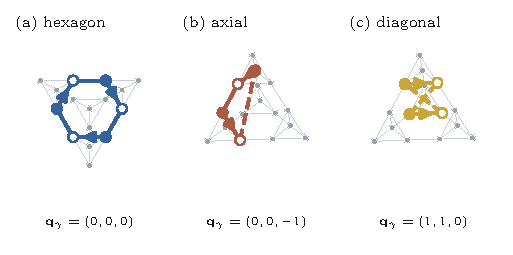
\includegraphics[width=0.92\textwidth]{fig_geometry.pdf}
  \caption{The finite-cluster geometry used by the implementation.  The
  stored bond images distinguish a loop that closes only through a periodic
  image from a contractible bulk hexagon, even when both look closed after
  wrapping sites into the simulation cell.}
  \label{fig:geometry}
\end{figure}

\section{Three levels that must not be conflated}

\fbox{\begin{minipage}{0.94\textwidth}
\textbf{Nonperturbative definition.}
Diagonalize the transported-dipole source family $H(\bm\theta)$, identify its
isolated ice-descended band, pull every source point into one ice basis with
the polar/Kato map, and take a controlled $M\to\infty$ character limit.

\textbf{Current production calculation.}
The active campaign extracts the exact 90-state cubic-16 band in the
12,870-dimensional $S^z=0$ sector at each independent character point.  It
uses the primitive $\bq=2\bm\delta$ source, matched $M=2,3,4$ grids, and the
exact 65,536-level microscopic complement for all-temperature observables.

\textbf{Not yet demonstrated.}
The repository has not established full-Hamiltonian FCC-32 thermodynamics,
cluster convergence, an unrestricted gap across all conserved magnetization
sectors, or matched QMC-SAC dynamics.  The converged cubic-16 heat and entropy
curves still fail their QMC tolerances.
\end{minipage}}

This distinction is the most important reading rule for both the manuscript
and the code.  The formal construction explains what a converged method would
mean.  The low-order rows explain the mechanism; they do not generate the
production spectrum.

\section{Geometry and basis construction}

\subsection{Periodic covering data}

Each site has a home-cell position $\bm r_i$, and the rows of $L$ are the
three supercell vectors.  Each nearest-neighbor bond stores an integer image
$\bm n_{ij}$.  Its displacement in the covering lattice is therefore
\begin{equation}
 \bm d_{ij}=\bm r_j-\bm r_i-\bm n_{ij}^{T}L.
 \label{eq:liftedbond}
\end{equation}
The spin bit pattern alone is insufficient: it forgets which periodic image a
virtual hop traversed.  The bond image must be propagated through every
intermediate state.

The geometry builder performs the following steps:
\begin{enumerate}
 \item generate wrapped site positions and supercell vectors;
 \item find nearest-neighbor bonds and their image vectors;
 \item enumerate tetrahedra from the adjacency graph;
 \item enumerate bit states satisfying two-in/two-out on every tetrahedron;
 \item enumerate ice-preserving simple four- and six-cycles; and
 \item lift each cycle to classify its winding.
\end{enumerate}
The resulting census is
\begin{center}
\begin{tabular}{lrrrr}
\toprule
cluster & ice states & winding 4 & contractible 6 & wrapping 6\\
\midrule
cubic-16 & 90 & 36 & 16 & 48\\
FCC-32 & 2970 & 24 & 32 & 96\\
\bottomrule
\end{tabular}
\end{center}
Neither cluster contains a contractible four-cycle.

\subsection{Bit basis and excitation energy}

A spin configuration is stored as an unsigned integer.  Bit $i=1$ denotes
$S_i^z=+1/2$.  For a tetrahedron $t$, let $n_t$ be the number of set bits.
After subtracting the common ice energy and setting $\Jzz=1$, the relative
Ising energy used in denominators is
\begin{equation}
 E_0(s)=\frac12\sum_t(n_t-2)^2.
 \label{eq:isingenergy}
\end{equation}
Thus every ice state has zero relative energy, while a state with spin-ice
charges has positive energy.  The recursive ice-state enumerator prunes a
partial bit assignment as soon as a tetrahedron can no longer reach exactly
two up spins.

\section{A virtual path is a data object}

The core numerical idea is not a matrix manipulation after the fact.  It is a
path-resolved construction in which every active row carries
\begin{equation}
 (s_{\rm current},\; a_{\rm source},\;\bm N,\;c).
\end{equation}
Here $s_{\rm current}$ is the current microscopic bit state,
$a_{\rm source}$ labels the initial ice basis state, $\bm N\in\mathbb Z^3$ is
the accumulated bond-image transport, and $c$ is the perturbative amplitude
including all denominators accumulated so far.

For every antiparallel nearest-neighbor pair, the perturbation flips both
bits.  The code contributes a factor $-1$ for the operator in Eq.~\eqref{eq:model};
the power of $\Jpm$ is inserted only when the final row table is assembled.
Depending on whether the active term is $S_i^+S_j^-$ or $S_i^-S_j^+$, the
stored image is updated by $+\bm n_{ij}$ or $-\bm n_{ij}$.

Rows may interfere, so duplicates are summed.  The merge key is
\begin{equation}
 (a_{\rm source},b_{\rm target},N_x,N_y,N_z),
 \label{eq:mergekey}
\end{equation}
not merely $(a_{\rm source},b_{\rm target})$.  Merging without $\bm N$ would
irreversibly combine contractible and winding contributions before they can
be projected.

\section{What the order-three routine computes}

Let $Q=1-P$ and define the reduced resolvent, with the ice energy set to zero,
\begin{equation}
 R=-QH_0^{-1}Q.
\end{equation}
Because $PVP=0$ for this model, the active row routine constructs
\begin{align}
 H_P^{(2)}&=PVRVP,\\
 H_P^{(3)}&=PVRVRVP.
 \label{eq:order23}
\end{align}
In code, division by
\code{-e1} or \code{-e2} applies one factor of $R$.  A path that has already
returned to the ice manifold after two hops is recorded in $H_P^{(2)}$ and is
not passed through a zero denominator into the third-order table.

The following pseudocode mirrors \code{sw\_order23}:
\begin{lstlisting}[language=Python]
for source, ice_state in enumerate(ice_basis):
    paths1 = apply_V([(ice_state, source, N=0, amplitude=1)])
    paths1.amplitude /= -ising_energy(paths1.state)

    paths2 = apply_V(paths1)
    returned = ising_energy(paths2.state) == 0
    H2_rows += project_to_ice(paths2[returned])

    charged2 = paths2[~returned]
    charged2.amplitude /= -ising_energy(charged2.state)
    paths3 = apply_V(charged2)
    H3_rows += project_to_ice(paths3[ising_energy(paths3.state) == 0])

H2_rows = merge_by_source_target_and_image(H2_rows)
H3_rows = merge_by_source_target_and_image(H3_rows)
\end{lstlisting}

This routine is a direct implementation of Eq.~\eqref{eq:order23}; it is not
an arbitrary-order Schrieffer--Wolff engine.  The all-order protocol instead
fixes the canonical, off-diagonal anti-Hermitian generator
\begin{equation}
 S^{(N)}=\sum_{n=1}^{N}\lambda^nS_n,
 \qquad PS_nP=QS_nQ=0,
\end{equation}
so that $Qe^{-S^{(N)}}He^{S^{(N)}}P=O(\lambda^{N+1})$.  At each order the
off-diagonal Baker--Campbell--Hausdorff coefficient $B_n$ gives
\begin{equation}
 S_n=-\mathcal L_0^{-1}(B_n),\qquad \mathcal L_0(X)=[H_0,X].
 \label{eq:swrecursion}
\end{equation}
Implementing Eq.~\eqref{eq:swrecursion} at order four is the next order
gate~\cite{Bravyi2011}.

\section{Transported dipole and the zero-transport selector}

For a completed row $a\to b$, let ``raised'' be sites that are down in $a$
and up in $b$, and ``lowered'' the reverse.  The implementation computes
\begin{equation}
 \bm\delta_{ba}=
 \sum_{i\in\mathrm{raised}}\bm r_i
 -\sum_{j\in\mathrm{lowered}}\bm r_j
 +\bm N^TL.
 \label{eq:delta}
\end{equation}
Coordinates and supercell vectors are multiplied by four and rounded to
integers before this calculation.  This is exact for the pyrochlore
coordinates used here and avoids floating-point equality tests.  The factor
of four changes units, not the condition $\bm\delta=0$.

For the exact character family, all completed ice-to-ice paths have even
components in these quarter-cell units.  The active code therefore uses the
primitive integer source $\bq=\bm\delta_4/2=2\bm\delta$.  Using
$\bq=\bm\delta_4$ would incorrectly alias the leading winding row on the
$M=2$ grid.

Changing a site's home-cell representative shifts the first two terms in
Eq.~\eqref{eq:delta} and $\bm N^TL$ oppositely.  Hence the transported dipole
and, in particular, its vanishing are invariant under this representation
choice.

The active assembler has two modes:
\begin{align}
 H_{\rm bare}^{(3)}&=\Jpm^2 H_P^{(2)}+\Jpm^3H_P^{(3)},\\
 H_{\rm clean}^{(3)}&=
 \sum_{\bm\delta=0}\left(\Jpm^2h^{(2)}(\bm\delta)
 +\Jpm^3h^{(3)}(\bm\delta)\right).
\end{align}
It then explicitly Hermitian-symmetrizes the dense ice-space matrix.  The
topology test verifies that the selector removes every winding four-loop and
retains every contractible hexagon on both clusters.

\section{Why this is a character projection}

Attach a phase $e^{i\btheta\cdot\Delta\bq}$ to each lifted hop.  Completed
rows have a finite Fourier expansion
\begin{equation}
 [H_P^{(N)}(\btheta)]_{ba}
 =\sum_{\bq}h_{ba}^{(N)}(\bq)e^{i\btheta\cdot\bq}.
\end{equation}
Average over the characters of $\mathbb Z_M^3$:
\begin{equation}
 \PP_M[H]=\frac{1}{M^3}
 \sum_{m_x,m_y,m_z=0}^{M-1}
 H\!\left(\frac{2\pi}{M}\bm m\right).
 \label{eq:characterprojector}
\end{equation}
Discrete Fourier orthogonality gives
\begin{equation}
 \PP_M[H_P^{(N)}]=
 \sum_{\bq=0\ ({\rm mod}\ M)}h^{(N)}(\bq).
 \label{eq:alias}
\end{equation}
At fixed perturbative order only finitely many transports are possible.  An
$M$ larger than every possible component therefore makes
Eq.~\eqref{eq:characterprojector} exactly equivalent to the direct
$\bm\delta=0$ row selector used by the active low-order code.  At all orders,
however, finite $M$ aliases $\bq=M\bm k$ with zero transport.  A controlled
$M\to2M$ ladder is required.

This also explains why several tempting operations are not equivalent:
\begin{itemize}
 \item Averaging $Z(\btheta)=\mathrm{Tr}\,e^{-\beta H(\btheta)}$ averages a
 nonlinear thermal quantity, not a Hamiltonian block.
 \item Averaging the microscopic Hamiltonian before multiplication projects
 individual hops, preventing the virtual paths from composing first.
 \item Deleting entries of the final ice-space matrix after image labels have
 been merged cannot recover the decomposition in Eq.~\eqref{eq:alias}.
 \item A fitted counterterm can cancel a chosen leading matrix element but
 does not classify all completed paths at higher order.
\end{itemize}

\section{Exact isolated-band continuation}

Suppose the microscopic Hamiltonian has an isolated exact band projector
$P_\lambda$ with $\mathrm{rank}(P_\lambda)=\mathrm{rank}(P)$.  The polar map
\begin{equation}
 W_\lambda=P_\lambda P(PP_\lambda P)^{-1/2}
 \label{eq:polar}
\end{equation}
canonically transports the model-space basis into the exact band.  It fixes
the otherwise arbitrary unitary gauge among eigenvectors in that band.  The
exact pulled-back operator is
\begin{equation}
 H_{\rm band}=W_\lambda^\dagger H W_\lambda.
\end{equation}

If $\Psi$ is a matrix of exact band eigenvectors and $X=P\Psi$, the code
orthonormalizes $X$ as
\begin{equation}
 q=X(X^\dagger X)^{-1/2},\qquad
 H_{\rm band}=q\,\mathrm{diag}(E_a)q^\dagger.
\end{equation}
It reports the minimum, mean, and maximum eigenvalues of $X^\dagger X$ and a
unitarity residual.  A singular projected Gram matrix means the selected band
cannot be canonically identified with the ice manifold; this is a failed
band-overlap gate, not a numerical nuisance to regularize away.

For a character calculation, Eq.~\eqref{eq:polar} must be applied separately
at each $\btheta$ before averaging operators.  Averaging eigenvalues alone
loses matrix character, while averaging eigenvectors without the polar gauge
mixes arbitrary basis choices.  The utility functions implementing the polar
map and operator average are present in \code{src/qsi\_campaign/protocol.py}
and are called by the active nonperturbative campaign.  At
$\Jpm/\Jzz=0.046$, the zero-source minimum overlap is 0.762; every generic
$M=3,4$ point has a larger minimum overlap.

\section{Full-temperature spectral replacement}

A low-energy effective block alone cannot produce all-temperature
thermodynamics.  The current cubic-16 construction retains the exact
microscopic complement.  Let the sorted exact spectrum be
$E_1\le\cdots\le E_{65536}$ and let $\widetilde E_1,\ldots,\widetilde E_{90}$
be the exact character-projected band spectrum.  First shift the clean band so
that its mean equals that of the lowest 90 exact levels, and then define
\begin{equation}
 \mathrm{spec}(H_{\rm replacement})=
 \{\widetilde E_a\}_{a=1}^{90}\cup\{E_i\}_{i=91}^{65536}.
 \label{eq:replacement}
\end{equation}
Trace matching fixes the band's scalar energy relative to the untouched
complement; specific heat within an isolated band would not fix this offset.

There is an important qualification.  The exact band is overlap-certified
within the conserved $S^z=0$ sector, where the zero-source gap above it is
$0.627\Jzz$.  The cached full spectrum gives a smaller unrestricted gap
$0.387\Jzz$ because other magnetization sectors are present.  Those sectors
do not mix with the ice band, but an unrestricted spectral-gap statement must
still report them separately.

For any finite spectrum, the thermodynamics are evaluated after shifting by
the ground-state energy to stabilize the Boltzmann weights:
\begin{align}
 Z'&=\sum_i e^{-\beta(E_i-E_0)},\\
 \langle E\rangle&=E_0+
 \frac{\sum_i(E_i-E_0)e^{-\beta(E_i-E_0)}}{Z'},\\
 C&=\frac{\langle(E-E_0)^2\rangle-
 \langle E-E_0\rangle^2}{T^2},\\
 S&=\ln Z'+\beta\langle E-E_0\rangle.
\end{align}
All extensive quantities are divided by the number of sites.  The temperature
grid is logarithmic from $10^{-4}\Jzz$ to $2\Jzz$ with 1400 points.

\section{External verification against Huang et al.}

Huang, Deng, Wan, and Meng simulate Eq.~\eqref{eq:model} at the sign-free
point $\Jpm/\Jzz=0.046$ using continuous-time worm QMC
\cite{Huang2018}.  This is an especially useful reference because its sign
and coupling convention match the repository directly.

The heat-capacity and entropy curves are extracted from the original vector
paths in Fig.~1(b) of the arXiv source.  The extractor records explicit axis
calibrations and writes a CSV with estimated digitization uncertainties.  The
comparison metric interpolates the finite-cluster curve on $\log T$ and then
computes an RMSE over the reference points.  Peak gates use fixed temperature
windows and log-position errors.

\begin{figure}[ht]
  \centering
  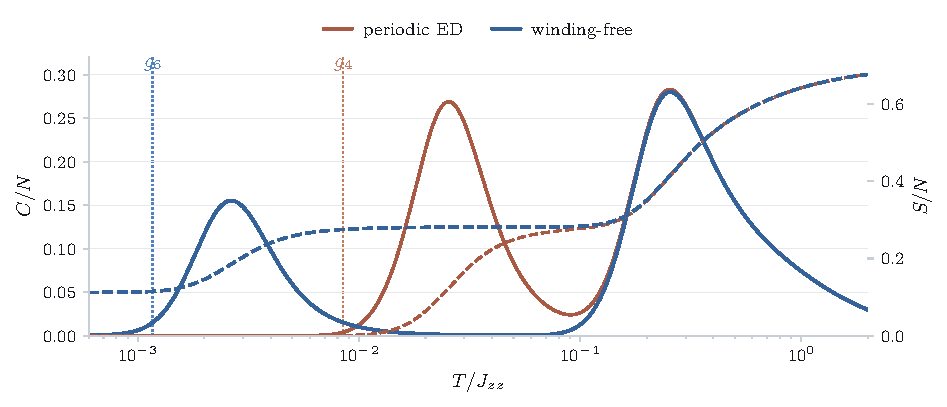
\includegraphics[width=0.95\textwidth]{fig_nonperturbative.pdf}
  \caption{Exact-band benchmark at $\Jpm/\Jzz=0.046$.  The $M=3,4$
  operators agree, while both converged thermodynamic curves remain distinct
  from QMC.}
  \label{fig:validation}
\end{figure}

The current numerical summary is
\begin{center}
\begin{tabular}{lccc}
\toprule
quantity & bare cubic-16 & clean cubic-16 & QMC\\
\midrule
low $T_{\rm p}/\Jzz$ & 0.02554 & 0.001463 & 0.001100\\
low-$T$ $C/N$ RMSE & 0.0859 & 0.02327 & 0\\
high $T_{\rm p}/\Jzz$ & 0.2549 & 0.2549 & 0.2105\\
$S/N$ RMSE & 0.0514 & 0.04509 & 0\\
\bottomrule
\end{tabular}
\end{center}
The converged $M=4$ low-temperature heat-capacity RMSE is reduced by 72.9\%,
but $0.02327$ remains above the threshold 0.02.  Its entropy RMSE $0.04509$
also fails.  Removing winding transfer does not guarantee correct
finite-cluster state counting or degeneracy, so these failures diagnose the
cluster rather than a lack of character convergence.

The same QMC paper supplies a future dynamical benchmark from stochastic
analytic continuation.  It reports the sublattice traces
\begin{equation}
 S^{zz}(\bm q,\omega)=\sum_{\alpha=1}^{4}
 S^{zz}_{\alpha\alpha}(\bm q,\omega),\qquad
 S^{+-}(\bm q,\omega)=\sum_{\alpha=1}^{4}
 S^{+-}_{\alpha\alpha}(\bm q,\omega)
\end{equation}
at $T/\Jzz=0.001$, $0.04$, and $0.1$.  A valid ED comparison must use only
momenta in the finite cluster's translation group, match the sublattice trace
and spin normalization, use a linear frequency axis, and state its broadening.
This dynamics gate remains pending.

\section{How the campaign runner fits together}

The production data path is short enough to audit directly:
\begin{lstlisting}[language=Python]
T = geomspace(1e-4, 2.0, 1400)

H0, Psi0 = exact_low_band(H(theta=0), dimension=90)
h0 = polar_pullback(H0, Psi0, ice_basis)
h2 = average(exact_gauge_orbit(h0, M=2))

for M in [3, 4]:
    for conjugation representative theta in Z_M^3:
        E, Psi = eigsh(H(theta), lowest=91)
        verify gap, Ritz residual, and ice overlap
        h[theta] = polar_pullback(E[:90], Psi[:, :90], ice_basis)
        h[-theta] = conjugate(h[theta])
    hM = average(h over Z_M^3)

E_full = load cached exact cubic16 spectrum
E_replacement = replace_low_band(E_full, eigvalsh(hM))
compute C/N and S/N from E_full and E_replacement

load Huang vector-extracted C/N and S/N
evaluate fixed gates
write nonperturbative operators, curves, caches, and report
\end{lstlisting}

No fitting parameter is adjusted in this sequence.  The model coupling is
fixed to the QMC value and no counterterm or perturbative coefficient enters
the production operator.

\section{Code map}

\begin{tabularx}{\textwidth}{p{0.32\textwidth}X}
\toprule
file or function & responsibility\\
\midrule
\nolinkurl{notes/recompute_finite_size_artifact.py} & active geometry, ice basis,
cycle census, virtual hopping, order-two/order-three row tables, transported
dipole, and dense assembly\\
\code{build\_cluster} & positions, bonds, image vectors, tetrahedra, loops,
and ice states\\
\code{apply\_v} & spin exchange, amplitude sign, and image-transport update\\
\code{merge\_rows} & coherent sum at fixed source, target, and image vector\\
\code{sw\_order23} & explicit $PVRVP$ and $PVRVRVP$ row construction\\
\code{transport\_delta} & integer form of Eq.~\eqref{eq:delta}\\
\code{assemble} & bare or direct zero-transport order-three matrix\\
\nolinkurl{src/qsi_campaign/protocol.py} & polar pullback, character average,
centered operator error, and low-band spectral replacement\\
\nolinkurl{src/qsi_campaign/exact_band.py} & fixed-magnetization basis,
microscopic character Hamiltonian, sparse exact-band extraction, gauge orbit,
and overlap/Ritz diagnostics\\
\nolinkurl{src/qsi_campaign/thermodynamics.py} & stable $E/N$, $C/N$, and $S/N$
from a finite spectrum\\
\nolinkurl{src/qsi_campaign/benchmarks.py} & vector-data loading and log-grid RMSE\\
\nolinkurl{campaign/data/extract_huang2018.py} & reproducible vector extraction of
Huang et al. Fig.~1(b)\\
\nolinkurl{campaign/run_nonperturbative.py} & active exact $M=2,3,4$ campaign,
restartable point cache, thermodynamics, and gate report\\
\nolinkurl{campaign/run_validation.py} & perturbative topology and cluster-size diagnostic\\
\nolinkurl{campaign/make_figures.py} & figures generated only from saved campaign
products\\
\bottomrule
\end{tabularx}

\section{Current gates and their interpretation}

\begin{center}
\small
\begin{tabularx}{\textwidth}{p{0.25\textwidth}p{0.16\textwidth}X}
\toprule
gate & status & interpretation\\
\midrule
loop topology & pass & winding four-loops removed; contractible hexagons retained\\
all-temperature stability & pass & high-$T$ peak position unchanged on cubic-16\\
QMC heat capacity & fail & exact $M=4$ low-$T$ RMSE $0.02327>0.02$\\
QMC entropy & fail & exact $M=4$ RMSE $0.04509>0.02$\\
fixed-$S^z$ band gap & pass & minimum source-resolved gap exceeds $0.627\Jzz$\\
band overlap & pass & minimum exact-band ice overlap is 0.762\\
character resolution & pass & centered $M=3\to4$ error is 0.498\%\\
order convergence & diagnostic only & order 2/3 is not the production method\\
QMC-SAC dynamics & pending & matched $S^{zz}$ and $S^{+-}$ not computed\\
FCC-32 full Hamiltonian & pending & current FCC-32 result is ice-manifold order three\\
\bottomrule
\end{tabularx}
\normalsize
\end{center}

All active grids use the same primitive $\bq=2\bm\delta$ source.  The large
$M=1\to2$ and 6.78\% $M=2\to3$ changes show why a single parity mask is not
enough; the 0.498\% $M=3\to4$ change supplies the first passed exact-band
character gate.

\begin{figure}[ht]
  \centering
  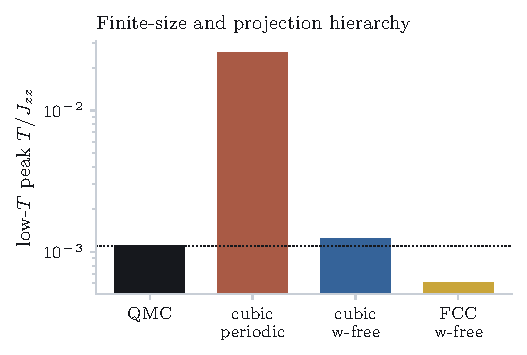
\includegraphics[width=0.92\textwidth]{fig_hierarchy.pdf}
  \caption{Validation hierarchy.  Topological correctness at orders two and
  three is necessary but not sufficient; the external and convergence gates
  must be passed before material-level claims are made.}
  \label{fig:hierarchy}
\end{figure}

\section{Common implementation mistakes}

\begin{enumerate}
 \item \textbf{Discarding image transport too early.}  Rows must remain keyed
 by Eq.~\eqref{eq:mergekey} until after projection.
 \item \textbf{Calling the order-three block ``exact ED.''}  Its diagonalization
 is exact only for that truncated 90- or 2970-dimensional operator.
 \item \textbf{Calling FCC-32 a full-Hamiltonian result.}  The active FCC-32
 spectrum contains only the order-three ice block; the $2^{32}$ complement is
 absent.
 \item \textbf{Treating finite $M$ as an exact all-order projection.}  Finite
 characters select $\bq=0\pmod M$, not only $\bq=0$.
 \item \textbf{Tracking eigenvalues without eigenvectors.}  Exact-band
 identity requires spectral separation and a nonsingular projected Gram
 matrix.
 \item \textbf{Averaging thermal observables.}  Character projection is linear
 at the operator level; $e^{-\beta H}$ is nonlinear.
 \item \textbf{Comparing dynamics at arbitrary momenta.}  A finite cluster has
 a discrete reciprocal translation group.  Plot interpolation cannot create
 missing physical momenta.
 \item \textbf{Using a heat-capacity peak as the only gate.}  The present
 entropy failure already shows why curve shape and state counting matter.
\end{enumerate}

\section{Reproduction and extension checklist}

From the repository root, the active workflow is
\begin{lstlisting}
python -m pip install -e .
make all
make nonperturbative-m4
\end{lstlisting}
It regenerates the row-resolved campaign, runs the unit tests, builds figures,
and compiles the manuscript, Supplemental Material, and this note.  The
machine-readable exact results are
\code{campaign/outputs/nonperturbative\_cubic16\_p0p046000.npz} and its JSON
report.  Individual source points are cached under
\code{campaign/cache/nonperturbative\_points/}.

An extension should proceed in this order:
\begin{enumerate}
 \item optionally extend to $M=5$ as a tighter character check;
 \item include all conserved magnetization sectors in the unrestricted gap;
 \item diagnose the heat and entropy failures before interpreting the low-temperature
 peak as bulk convergence;
 \item match the QMC-SAC channels at the finite cluster's actual momenta; and
 \item only then deploy a stochastic-complement method on FCC-32 and proceed
 to a material fit.
\end{enumerate}

\section{Takeaway}

The protocol's useful idea is simple: a periodic image label is physical
bookkeeping for a virtual path, even though it is invisible in the wrapped
spin configuration.  Keeping that label until a completed path returns to the
ice band makes winding and contractible processes separable.  The present
implementation proves the path classification at orders two and three and
then executes the production projection with exact microscopic eigenspaces.
The $M=3,4$ agreement removes perturbative-order ambiguity from cubic-16.  The
remaining heat and entropy failures show that this converged finite cluster
still cannot support a bulk or material claim.

\bibliographystyle{unsrt}
\bibliography{../paper/references}

\end{document}
